\documentclass{fenicscourse}
%\documentclass{fenics}
%\usepackage{booktabs}
%\usepackage{caption}
\usepackage{xmpmulti}

% General math notation
\newcommand{\N}{\mathbb{N}}
\newcommand{\PP}{\mathbb{P}}
\newcommand{\QQ}{\mathbb{Q}}

% Math operators
\DeclareMathOperator{\ord}{ord}
\DeclareMathOperator{\Kern}{ker}
\DeclareMathOperator{\Image}{im}
\DeclareMathOperator{\spann}{span}
\DeclareMathOperator{\diam}{diam}


% Mesh and FEM notation
%\newcommand{\dx}{\, \mathrm{d} x}
%\newcommand{\ds}{\, \mathrm{d} s}
%\newcommand{\dS}{\, \mathrm{d} S}
\newcommand{\mesh}{\mathcal{T}}
\newcommand{\facets}{\mathcal{F}}
\newcommand{\inmesh}{\partial_i \mathcal{T}}
\newcommand{\exmesh}{\partial_e \mathcal{T}}

\newcommand{\jump}[1]{\llbracket #1 \rrbracket}
\newcommand{\avg}[1]{\langle #1 \rangle}
\newcommand{\meanvalue}[1]{\langle #1 \rangle}
\newcommand{\vect}[1]{\mathbf{#1}}

\newcommand{\gradhterm}[2]{(\nabla_h #1, \nabla_h #2)_{\Omega}}
\newcommand{\consterm}[2]{(\avg{\nabla_h #1} \dotn,\jump{#2})_{\inmesh}}
\newcommand{\penterm}[2]{( h^{-1} \jump{#1}, \jump{#2})_{\inmesh}}

\newcommand{\Ctr}{C_{\text{tr}}}

% Abbreviations for names etc
\newcommand{\apriori}{\emph{a~priori}}
\newcommand{\aposteriori}{\emph{a~posteriori}}

% Dimensions
\newcommand{\codesize}{\footnotesize}

% Environments
\DefineVerbatimEnvironment{code}{Verbatim}{frame=single,rulecolor=\color{blue}}

% Notes
\newcommand{\amnote}[1]{\todo[inline,color=blue!40]{\underline{AM:} #1}}
\newcommand{\mglnote}[1]{\todo[inline,color=red!40]{\underline{MGL:} #1}}
\newcommand{\alnote}[1]{\todo[inline,color=green!40]{\underline{AL:} #1}}
\newcommand{\mernote}[1]{\todo[inline,color=pink!40]{\underline{MER:} #1}}

% Special notation PI
\newcommand{\OmegaD}{\Omega_{0,\mathrm{D}}}
\newcommand{\OmegaN}{\Omega_{0,\mathrm{N}}}
\newcommand{\OmegaO}{\Omega_{_\mathrm{O}}}
\newcommand{\bfsigma}{{\pmb\sigma}}
\newcommand{\bfepsilon}{{\pmb\epsilon}}

% Special notation for PII
\newcommand{\bfu}{\boldsymbol{u}}
\newcommand{\bff}{\boldsymbol{f}}
\newcommand{\bfg}{\boldsymbol{g}}
\newcommand{\bfv}{\boldsymbol{v}}
\newcommand{\bfe}{\boldsymbol{e}}
\newcommand{\bfn}{\boldsymbol{n}}
\newcommand{\bfx}{\boldsymbol{x}}
\newcommand{\Oast}{\Omega^{\ast}}
\newcommand{\Vast}{\mathcal{V}^{\ast}}

%\newcommand{\meshast}{\mathcal{T}_{\ast}}
\newcommand{\pO}{\partial \Omega}
\newcommand{\meshast}{\mathcal{T}^{\ast}}
\newcommand{\Fast}{\mathcal{F}^{\ast}_{\Gamma}}
\newcommand{\piast}{\pi^{\ast}_h}
\newcommand{\tnast}{\tn_{\ast}}
\newcommand{\tnsip}{\tn_{\text{sip}}}
\newcommand{\tnsipast}{\tn_{\text{sip},\ast}}
\newcommand{\asip}{a^{\text{sip}}_h}

\newcommand{\mcF}{\mathcal{F}}
\newcommand{\mcT}{\mathcal{T}}
\newcommand{\mcV}{\mathcal{V}}
\newcommand{\mcE}{\mathcal{E}}
\newcommand{\mcN}{\mathcal{N}}
\newcommand{\mcC}{\mathcal{C}}
\newcommand{\mcA}{\mathcal{A}}
\newcommand{\tn}{|\mspace{-1mu}|\mspace{-1mu}|}
\newcommand{\Pzero}{P_h^{0,\mathrm{dc}}}
\newcommand{\Pone}{P_h^1}
\newcommand{\ndot}{\bfn \cdot}
\newcommand{\dotn}{\cdot \bfn}
\newcommand{\bfw}{\boldsymbol{w}}
\newcommand{\Wspace}{{\mathcal{V}_h}}

% Special notation for PIII
\newcommand{\nablan}{\partial_{\bfn}}
\newcommand{\OmcupOm}{\Omega_1 \cup \Omega_2}
\newcommand{\mcupm}{{\mathcal{T}^{\ast}_1} \cup \mesh_2}
%\newcommand{\mcupm}{{\meshast}_1 \cup \mesh_2}
%\newcommand{\meanvalue}[1]{\langle #1 \rangle_{\alpha}}
\newcommand{\ifnormalpha}[1]{\ifnorm{#1}{\alpha}}
\newcommand{\ifnorm}[2]{\| #1 \|_{#2,h,\Gamma}}
\newcommand{\tildev}{\widetilde{\bfv}}
\newcommand{\bfphi}{\boldsymbol{\phi}}
\newcommand{\picorr}{\pi^c}

% Math macros
\newcommand{\renni}[2]{\langle #2 ,\; #1 \rangle}


\tikzstyle{na} = [baseline=-.5ex]

\tikzstyle{every picture}+=[remember picture]
\everymath{\displaystyle}

\mode<presentation> {\setbeamercovered{invisible}}

\begin{document}

\fenicslecture{Lecture 11: A posteriori error estimates and adaptivity}
              {Andr\'e Massing\\
              Marie Rognes \\
              Anders Logg}

\linespread{1.5}

% Repeat a priori estimates
\begin{frame}[t]
  \frametitle{\emph{A priori} estimates}
    If $u \in H^{k+1}(\Omega)$ and $V_h = P^k(\mcT_h)$ then
    \begin{gather*}
      \tn u - u_h \tn \leqslant C h^{k} \| u \|_{\Omega, k+1} \\
      \| u - u_h \|_{L^2(\Omega)} \leqslant C h^{k+1} \| u \|_{\Omega, k+1}
    \end{gather*}
  \begin{columns}[c]
    \begin{column}{0.4\textwidth}
    \multiinclude[graphics={width=1.0\textwidth},format=png]{png/mesh-ref}
    \end{column}
    \begin{column}{0.6\textwidth}
    \only<2>{
      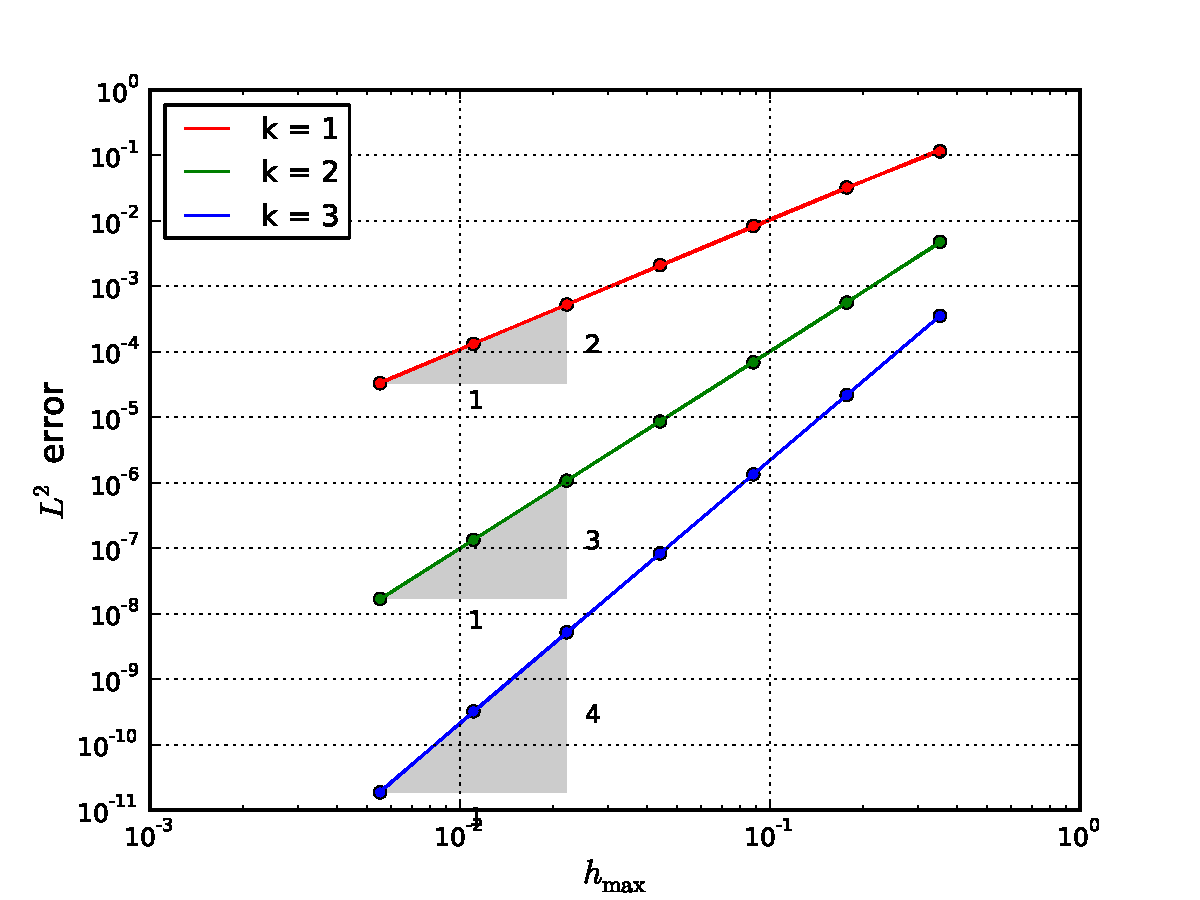
\includegraphics[width=1.0\textwidth]{pdf/l2-convergence.pdf}
    }
    \only<3>{
      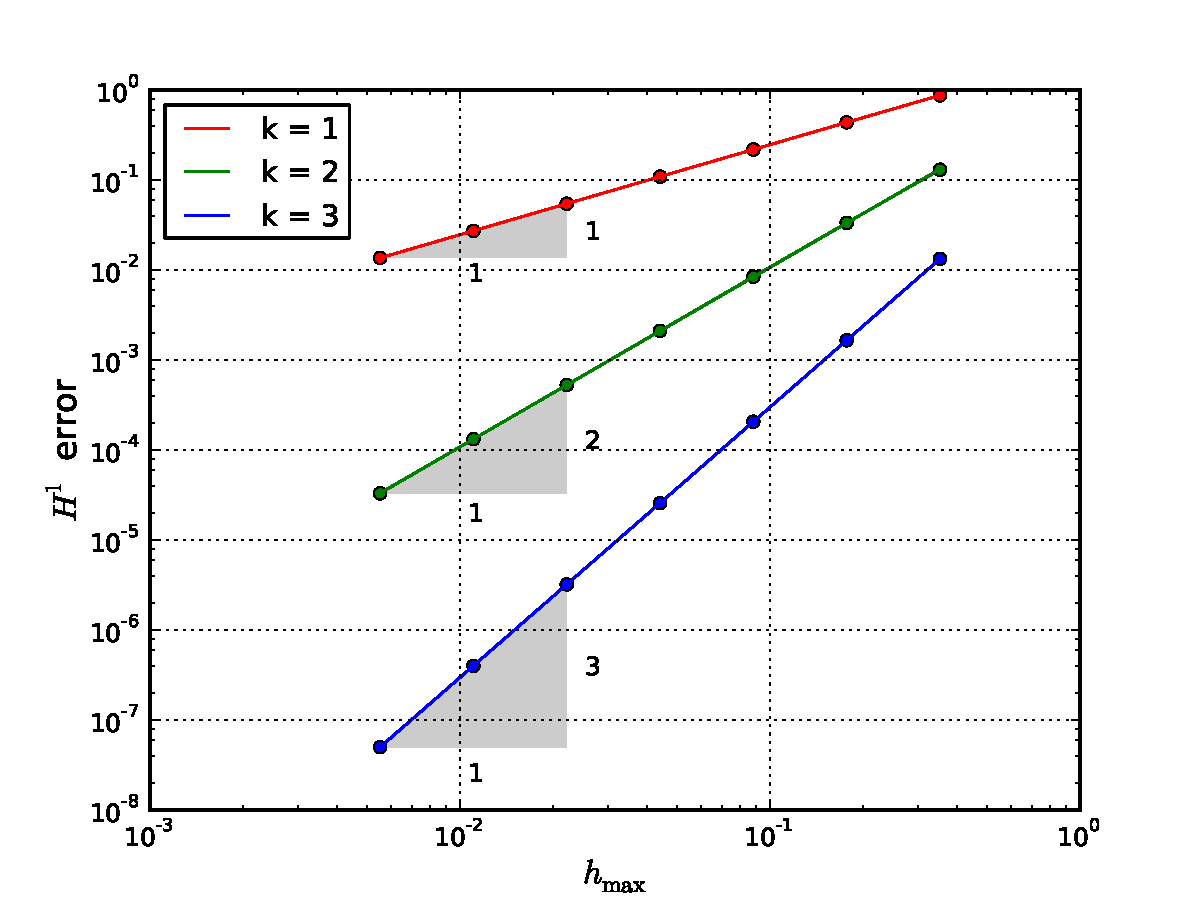
\includegraphics[width=1.0\textwidth]{pdf/h1-convergence.pdf}
    }
    \end{column}
  \end{columns}
%Figure left: mesh refinement \\
%Figure right: convergence plots for p = 1 2 3 \\
%Mention h vs p vs hp estimates. Mention paper by rivere ..
\end{frame}


% Motivate a posteriori error estimation
\begin{frame}
  \frametitle{Mesh adaptation can yield more accurate
  results with less computational resources}
  \begin{columns}
    \begin{column}{0.6\textwidth}
      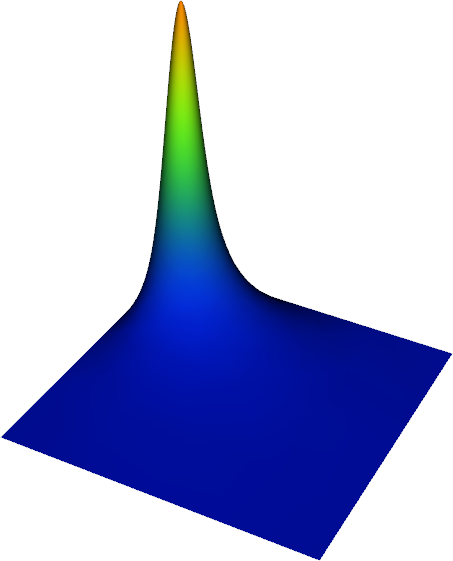
\includegraphics[width=0.9\textwidth]{png/exact-solution-alpha.png}
    \end{column}
    \begin{column}{0.4\textwidth}
    \end{column}
  \end{columns}
\end{frame}
%
\begin{frame}
  \frametitle{Mesh adaptation can yield more accurate
  results with less computational resources}
  \begin{columns}
    \begin{column}{0.6\textwidth}
    \only<1>{
      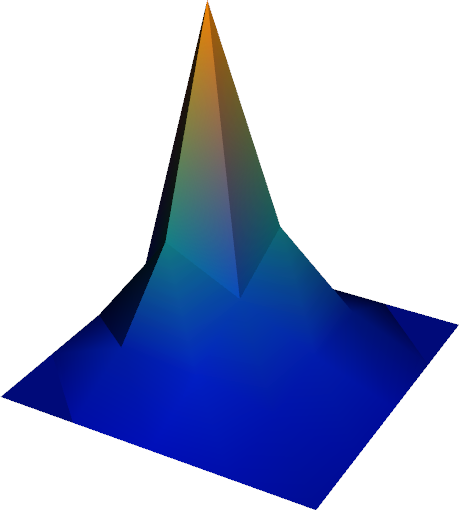
\includegraphics[width=0.9\textwidth]{png/solution-refinement-1.png}
    }
    \only<2>{
      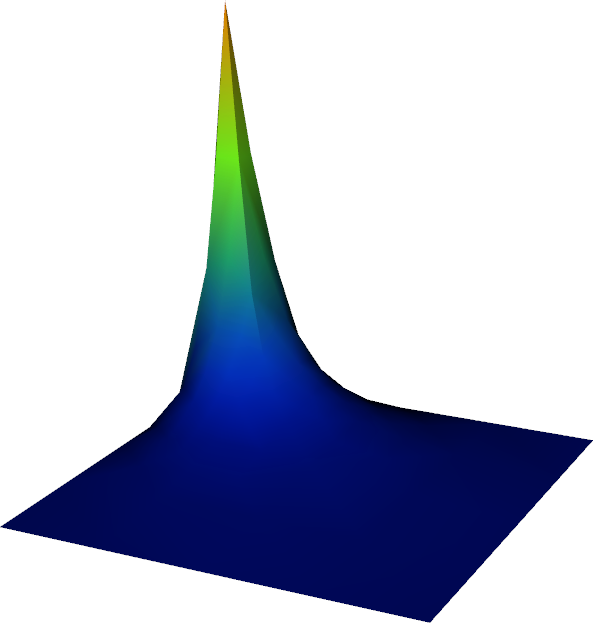
\includegraphics[width=0.9\textwidth]{png/solution-refinement-2.png}
    }
    \only<3>{
      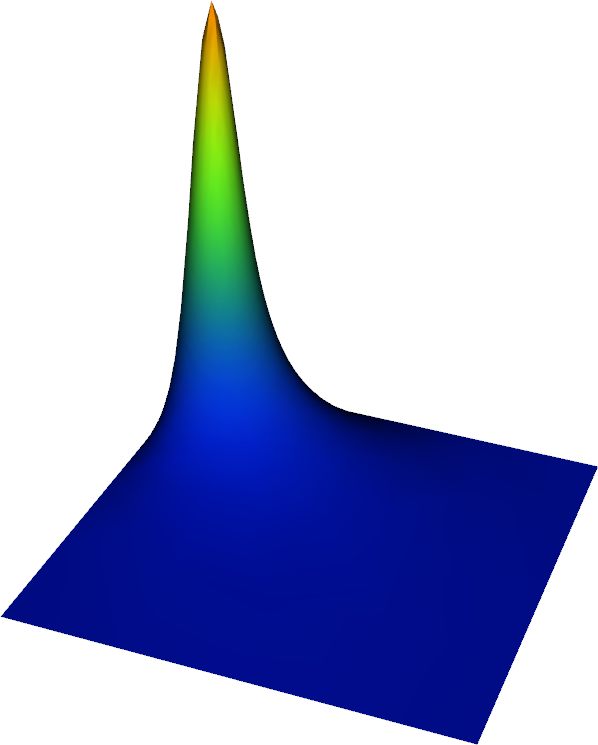
\includegraphics[width=0.9\textwidth]{png/solution-refinement-3.png}
    }
    \end{column}
    \begin{column}{0.4\textwidth}
      \multiinclude[graphics={width=1.0\textwidth,angle=-90},format=pdf,start=1]{pdf/mesh-refinement}
    \end{column}
  \end{columns}
\end{frame}

%  Start with introductory figure again. explain concept
%  of a posteriori estimate for both error assement
%  and driving refinement
%  \\
%  h vs. p refinement (or both)
%  need for error indicators, how do they look like
%  \\
%  they something about the advantage of DF for refinement 
%  and higer order elements
%  \\give versions of error indicators
%  \\mention work from Stamm 1, Houston (2 papers)
%  \\mention efficiency vs reliability


% Explain adaptivity steering circle
\begin{frame}
  \frametitle{Adaptive error control}
  \begin{center}
    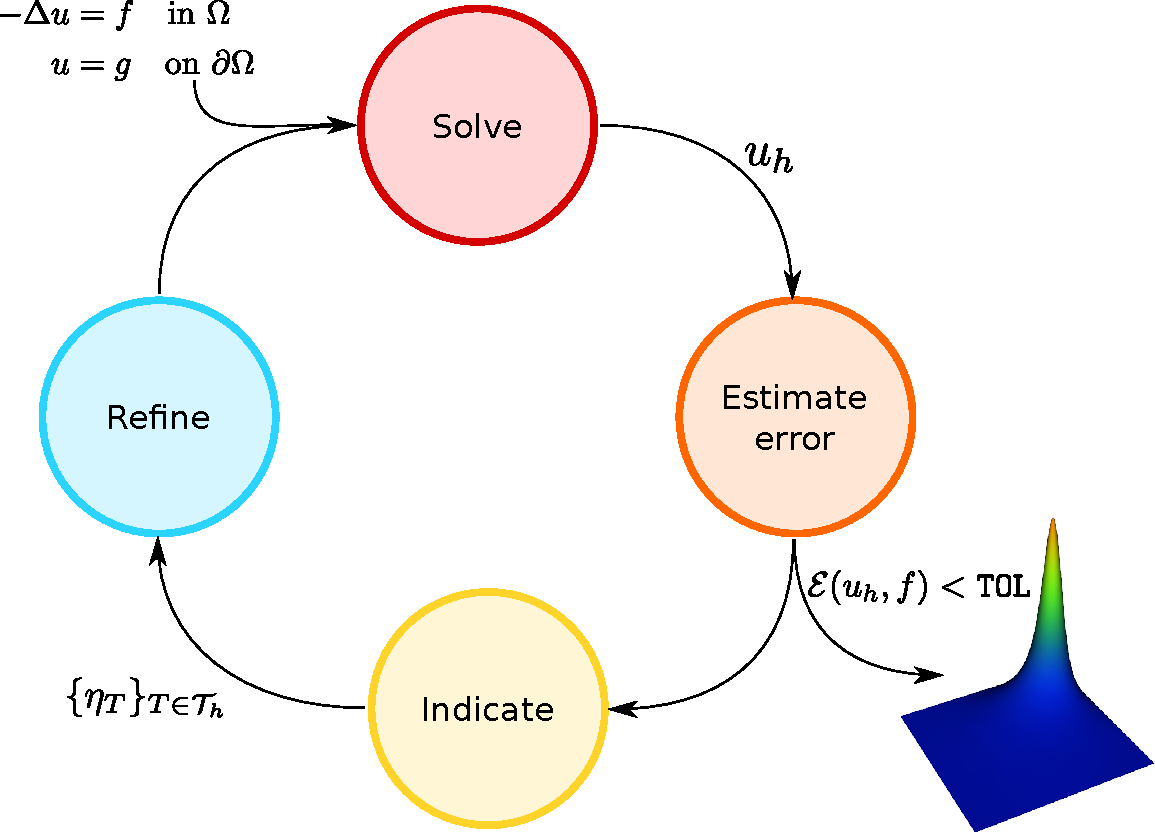
\includegraphics[width=0.9\textwidth]{pdf/h-adaptivity-workflow.pdf}
  \end{center}
\end{frame}


% Explain the different components

% A posteriori error estimation
\begin{frame}
  \frametitle{Desired properties of error estimators}
  An error estimator $\mathcal{E} \sim \| u - u_h \|$ has to be
      \begin{align*}
        &\text{\colemph{computable}} \quad  \mathcal{E} = \mathcal{E}(u_h,f)
        \\
        \intertext{and should be}
        &\text{\colemph{reliable}} \quad\tn u - u_{h} \tn \leqslant
        C \mcE(u_{h},f) \\
        &\text{\colemph{efficient}} \quad c \mcE(u_{h},f) \leqslant
        \tn u - u_{h} \tn  \\
        &\text{\colemph{local}} \quad\mcE(u_{h},f)^2 = \sum_{T\in
        \mesh_h} \rho_{T}(u_{h},f)^2  
      \end{align*}
%      \bigskip
  The quality of $\mathcal{E}(u_h, f)$ is measured by the
\colemph{efficiency index $\eta$} 
\[
  \eta(\mathcal{E}(u_h,f)) = \dfrac{\| u - u_h \|}{\mathcal{E}(u_h,f)}
\]
  If $\eta(\mathcal{E}(u_h,f)) \to 1$ as $h \to 0$, the error
  estimator is \colemph{asymptotically exact}.
\end{frame}


\begin{frame}
  \frametitle{Types of error estimators}
 
  \begin{itemize}
    \item Explicit residual-based error estimators
    \item \textcolor{grey}{Implicit error estimator based on local problems}
    \item \textcolor{grey}{Gradient recovery estimators}
    \item \textcolor{grey}{Hierarchic error estimators}
    \item Goal-oriented error estimators
  \end{itemize}

\end{frame}

\begin{frame}
  \frametitle{Explicit residual based error estimators}
  Model problem
  \begin{align*}
    -\Delta u &= f \quad \text{in } \Omega
    \\
    u &= 0  \quad \text{on } \partial \Omega
  \end{align*}
  Residual equation
  \begin{align*}
    R(u_h, f; v) = (\nabla (u - u_h), \nabla v) = (f, \nabla v) - (\nabla u_h,
    \nabla v)\quad \foralls v \in H^1_0(\Omega)
  \end{align*}
  Recall Galerkin orthogonality
  \[
    R(u_h, f; v_h) = 0 \quad \foralls v_h \in \widehat{V}_h
  \]
  Interpolation operator $\pi_h: V \to V_h$
  \begin{align*}
    R(v) &= (f ,v - \pi_h v) - (\nabla u_h, \nabla(v - \pi_h v)) \\
         &= \sum_{T \in \mesh_h} (f + \Delta u_h, v - \pi_h v)_T
    - \sum_{T \in \mesh_h} (\nabla u_h \cdot n_T, v -
    \pi_h)_{\partial T}
    \\
         &= \sum_{T \in \mesh_h} (f + \Delta u_h, v - \pi_h v)_T
    - \sum_{F \in \partial \mathcal{F}^i} (\jump{\nabla u_h \cdot
    n_T}, v - \pi_h)_{F}
  \end{align*}
\end{frame}
\begin{frame}
  \frametitle{Explicit residual based error estimators}
  Starting from
  \begin{equation*}
    R(v) = \sum_{T \in \mesh_h} (f + \Delta u_h, v - \pi_h v)_T
    - \sum_{F \in \partial \mathcal{F}^i} (\jump{\nabla u_h \cdot
    n_T}, v - \pi_h)_{F}
  \end{equation*}
  and using the quasi-interpolant by Clement, which satisfies
  \begin{align*}
    \| v - \pi_h \|_{0,T} \le C_1  h_T \| v \|_{\omega(T)} \\
    \| v - \pi_h \|_{0,F} \le C_2  h_F^{1/2} \| v \|_{\omega(F)},
  \end{align*}
  one obtains
  \begin{align*}
    |R(v)| \leqslant C \| v \|_1
  \left
\{
  \sum_{T \in \mesh_h} h_T^2 \|f + \Delta u_h \|^2 +
  \sum_{F \in \mathcal{F}^i} h_E \| \jump{\nabla u_h} \cdot n \|_F^2
  \right
\}^{1/2}
  \end{align*}
\end{frame}
\begin{frame}
  \frametitle{Explicit, residual based error estimators}
  Define
  \begin{alignat*}{3}
    &\text{\color{fenicsred}Element residual}\quad & & r_T := f + \Delta |_T \\
    &\text{\color{fenicsred}Facet residual}\quad & & r_F := \jump{\nabla u_h \cdot n} |_T \\
    &\text{\color{fenicsred}Error indicators} \quad  & &\rho_T^2 := h_T^2 \|r_T\|_T^2 +
    \dfrac{1}{2} \sum_{F \in \partial T} h_F \| r_F \|^2_T
  \end{alignat*}
  Poincar\'e inequality gives $\|v\|_1 \sim \| \nabla v \|$ an thus
  \begin{align*}
    \| u - u_h \|_1 &\leqslant \sup_{v \in V}\dfrac{(\nabla(u-u_h),\nabla v)}{\|
      v \|_1} = \sup_{v \in V} \dfrac{|R(v)|}{\|v\|_1}  \\
      & \leqslant C \big( \sum_{T \in \mesh_h} \rho_T^2 \big)^{1/2}
  \end{align*}
  proving the reliability of the error estimator defined by
  $\{\rho_T\}_T$.
\end{frame}


%\begin{frame}
    \frametitle{FEniCS coding interlude}
    Again, we look at the Poisson problem
    \begin{align*}
        -\Delta u &= e^{-100(x^2 + y^2)} \quad \text{in } \Omega \\
                u &= 0 \quad \text{on } \partial \Omega \\
    \end{align*}
    \vspace{-3em}
    \begin{columns}[c]
        \begin{column}{0.5\textwidth}
    Our mission is to implement the classical, residual-based error
    estimator and to solve this problem adaptively for a given
    tolerance $TOL=1.0e-3$. As marking strategy we choose to mark
    those $30 \%$ of elements with the largest element residual.
        \end{column}
        \begin{column}{0.5\textwidth}
    \begin{center}
        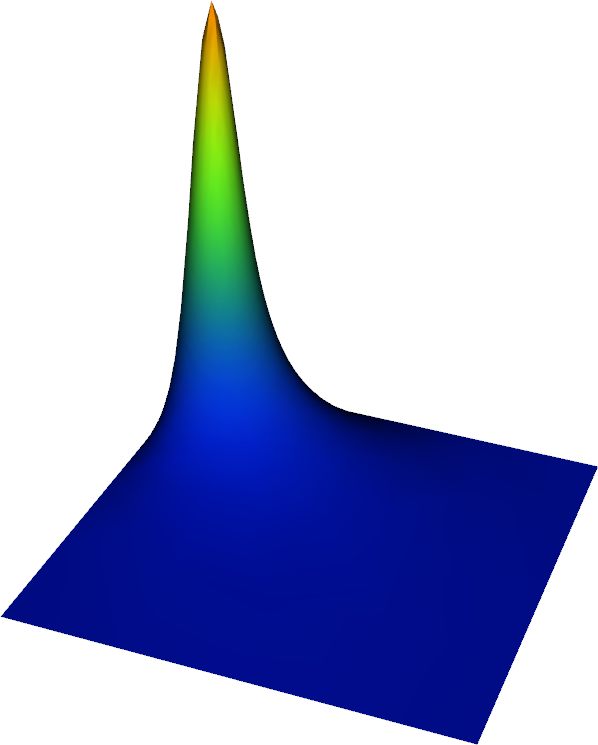
\includegraphics[width=0.8\textwidth]{png/solution-refinement-3.png}
    \end{center}
        \end{column}
    \end{columns}
\end{frame}


% TODO: Add
% Marking strategies
% Refinement strategies

% Goal-oriented adaptivity
\fenicssection{Goal-oriented error control}
\begin{frame}
  \frametitle{What is goal-oriented error control? \\
    {\small The scientist's viewpoint}}
  \begin{center}
    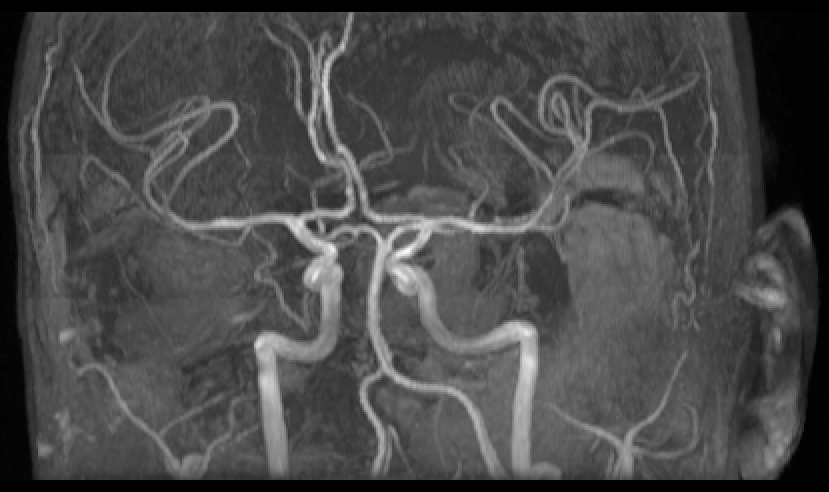
\includegraphics[height=3.5cm]{png/circle_of_willis_scan.png} \hspace{0.3cm}
    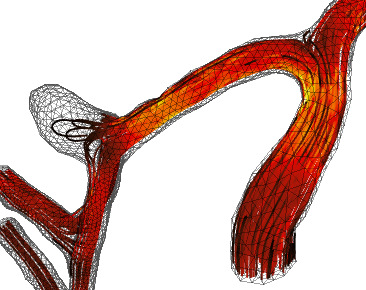
\includegraphics[height=3.5cm]{png/circle_of_willis_aneurysm.png}
    \\
    \vspace{3.0em}
    Shear stress at vessel wall?
  \end{center}
%    {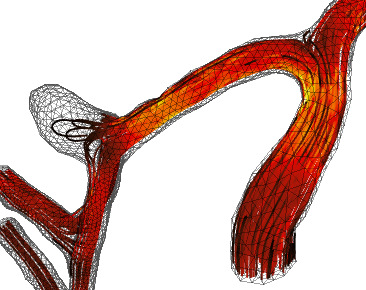
\includegraphics[width=0.4\textwidth]{png/circle_of_willis_aneurysm.png}};
%  \begin{tikzpicture}
%    \node at (0,1)
%    {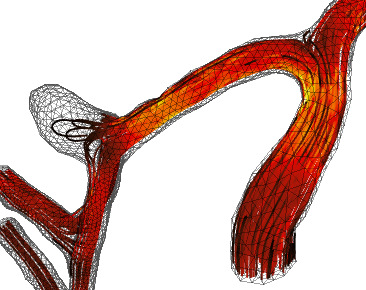
\includegraphics[width=0.4\textwidth]{png/circle_of_willis_aneurysm.png}};
%    \node at (5,-1){\includegraphics[width=0.6\textwidth]{/home/meg/presentations/slides/eps/vessel.png}};
%    \node at (5, 2){Quantity of interest:};
%    \node at (5, 1.5){Shear stress at vessel wall?};
%  \end{tikzpicture}
\btVFill
{\tiny [Valen-Sendstad '08]}
\end{frame}

\begin{frame}[fragile]
  \frametitle{What is goal-oriented error control?}
  \framesubtitle{The mathematician's viewpoint}

  \begin{block}{Input}
  {\small
  \begin{itemize}
  \item PDE: find $u \in V$ such that $a(u, v) = L(v) \quad
    \foralls v \in V$
  \item Quantity of interest/Goal: $\goal: V \rightarrow \R$
  \item Tolerance: $\epsilon > 0$
  \end{itemize}
  }
  \end{block}

  \begin{block}{Challenge}
    Find $V_h \subset V$ such that $|\goal(u) - \goal(u_h)| <
    \epsilon$ where $u_h \in V_h$ is determined by
    \begin{equation*}
      a(u_h, v) = L(v)  \quad \foralls v \in V_h
    \end{equation*}
  \end{block}
\end{frame}

%\begin{frame}[shrink=5]
\begin{frame}
  \frametitle{The error measured in the goal is the residual of the
    dual solution}
  \begin{enumerate}
    \item Recall residual
      $\qquad
    R(v) := L(v) - a(u_h, v)
    $
\item Introduce dual problem
    \vspace{-0.5em}
  \begin{equation*}
    \text{Find $z \in \widetilde{V}$:}  \quad a^* (z, v) = \goal(v)
    \quad \foralls v \in \widehat{V}
  \end{equation*}
  \item Dual solution + residual $\implies$ error
    \vspace{-0.5em}
    \begin{align*}
      \goal(u) - \goal(u_h)
      &=\goal(u - u_h)
      =a^{\ast}(z,u-u_h)
      =a(u-u_h, z)
      \\
      &= L(z) - a(u_h, z)
      = R(z) 
      = R(z - z_h)
      %= a^*(u, z) - a(z, u_h)
%      = L(z) - a(u_h, z)
%      = r(z) = r(z - z_h)
  \end{align*}
  \item A good dual approximation $\tilde z_h$ gives computable error
    estimate
    \vspace{-1.8em}
    \begin{equation*}
      \eta_h = r(\tilde z_h)
    \end{equation*}
  \item Error indicators ... ?
  \end{enumerate}

\end{frame}
\begin{frame}
  \frametitle{The dual-weighted residual method for the Poisson
  problem}
  Start with representation
  \begin{align*}
    |\goal(u) - \goal(u_h)| = |R(u-u_h,z-z_h)|.
  \end{align*}
  Integrate by parts as for the classical energy-norm estimate gives  
  \begin{align*}
    |\goal(u) - \goal(u_h) | 
    \leqslant \sum_{T \in \mesh_h} \rho_T \omega_T,
  \end{align*}
  where $\rho_T$ is resembles the standard element \colemph{residual}
  \vspace{-0.5em}
  \begin{align*}
    \rho_T = \| r_T \|_T + h^{1/2}_T \| r_F \|_{\partial T}\\
    \intertext{and $\omega_T$ is a \colemph{weight}}
    \omega_T = \| z - z_h \|_T + h^{1/2}_T \| z - z_h \|_{\partial T}
  \end{align*}
  derived from the \colemph{dual} solution $z$.
  
\end{frame}



\begin{frame}
  \frametitle{What is automated goal-oriented error control?}

  \begin{center}
    \tikzstyle{input}=[rectangle,fill=green!20,thick, draw=green!30,
      inner sep=10pt,minimum width=1.5cm, minimum height=1cm]
    \tikzstyle{process}=[rectangle, draw=black!50, fill=black!70, thick,
      inner sep=10pt,minimum width=3cm, minimum height=4cm]
    \tikzstyle{output}=[rectangle,fill=blue!20, draw=blue!10, thick,
      inner sep=10pt,minimum width=2mm, minimum height=2mm]
    \tikzstyle{into}=[->, shorten >=1pt, >=stealth, thick]
    \tikzstyle{outof}=[<-, shorten >=1pt, >=stealth, thick]

    \begin{tikzpicture}[bend angle=45, scale=.8]
      \node[process] (process) {};
      \node[input, node distance=4cm] (input goal) [left of=process]  {$\goal$}
      edge [into] (process);
      \node[input, node distance=1.5cm] (input eq) [above of=input goal]  {$F$}
      edge [into] (process);
      \node[input, node distance=1.5cm] (input tol) [below of=input goal]  {$\epsilon$}
      edge [into] (process);
      \node[output, node distance=4.5cm] (output) [right of=process]  {$\goal(u_h) \approx \goal(u) \pm \epsilon$}
      edge [outof] (process);
    \end{tikzpicture}
  \end{center}


\end{frame}

\begin{frame}[fragile]
  \frametitle{What is automated goal-oriented error control?}

  \begin{center}
    \tikzstyle{input}=[rectangle,fill=green!20,thick, draw=green!30,
      inner sep=10pt,minimum width=1.5cm, minimum height=1cm]
    \tikzstyle{process}=[rectangle, draw=black!50, fill=black!70, thick,
      inner sep=10pt,minimum width=3cm, minimum height=4cm]
    \tikzstyle{output}=[rectangle,fill=blue!20, draw=blue!10, thick,
      inner sep=10pt,minimum width=2mm, minimum height=2mm]
    \tikzstyle{into}=[->, shorten >=1pt, >=stealth, thick]
    \tikzstyle{outof}=[<-, shorten >=1pt, >=stealth, thick]

    \begin{tikzpicture}[bend angle=45, scale=.8]
      \node[process] (process) {};
      \node[input, node distance=4cm] (input goal) [left of=process]  {$\goal$}
      edge [into] (process);
      \node[input, node distance=1.5cm] (input eq) [above of=input goal]  {$a, L$}
      edge [into] (process);
      \node[input, node distance=1.5cm] (input tol) [below of=input goal]  {$\epsilon$}
      edge [into] (process);
      \node[output, node distance=4.5cm] (output) [right of=process]  {$\goal(u_h) \approx \goal(u) \pm \epsilon$}
      edge [outof] (process);
    \end{tikzpicture}


  \end{center}
  \begin{block}{FEniCS/DOLFIN}
    \vspace{-1em}
    \begin{python}
pde = VariationalProblem(a, L, bc)
pde.solve(u, tol, M)
    \end{python}
  \end{block}
\end{frame}

\begin{frame}[fragile]
  \frametitle{Automated goal-oriented adaptivity -- A complete example}
  \vspace{-2.0em}
\begin{python}
from fenics import *

# Create mesh and define function space
mesh = UnitSquareMesh(8, 8)
V = FunctionSpace(mesh, "Lagrange", 1)

# Define boundary condition
u0 = Function(V)
bc = DirichletBC(V, u0, "x[0] < DOLFIN_EPS || x[0] > 1.0 - DOLFIN_EPS")
\end{python}
\end{frame}


\begin{frame}[fragile]
  \frametitle{Automated goal-oriented adaptivity -- A complete example}
Define variational problem:
\vspace{-1.0em}
\begin{python}
u = TrialFunction(V)
v = TestFunction(V)
f = Expression("10*exp(-(pow(x[0] - 0.5, 2) + pow(x[1] - 0.5, 2)) / 0.02)",
               degree=1)
g = Expression("sin(5*x[0])", degree=1)
a = inner(grad(u), grad(v))*dx
L = f*v*dx + g*v*ds
\end{python}
\end{frame}

%\begin{frame}[fragile]
%  \frametitle{Automated goal-oriented adaptivity -- A complete example}
%\vspace{-1.0em}
%\begin{python}
%u = TrialFunction(V)
%v = TestFunction(V)
%f = Expression("10*exp(-(pow(x[0] - 0.5, 2) + pow(x[1] - 0.5, 2)) / 0.02)",
%               degree=1)
%g = Expression("sin(5*x[0])", degree=1)
%a = inner(grad(u), grad(v))*dx
%L = f*v*dx + g*v*ds
%\end{python}
%\end{frame}

\begin{frame}[fragile]
  \frametitle{Automated goal-oriented adaptivity -- A complete example}
Define function for the solution:
\vspace{-1.0em}
\begin{python}
u = Function(V)
\end{python}
\bigskip
Define goal functional (quantity of interest) and tolerance:
\vspace{-1.0em}
\begin{python}
M = u*dx
tol = 1.e-5
\end{python}
\end{frame}

\begin{frame}[fragile]
  \frametitle{Automated goal-oriented adaptivity -- A complete example}
Solve equation a = L with respect to u and the given boundary
conditions, such that the estimated error (measured in M) is less
than tol
\vspace{-1.0em}
\begin{python}
solver_parameters = {"error_control":
                     {"dual_variational_solver":
                      {"linear_solver": "cg"}}}
solve(a == L, u, bc, tol=tol, M=M, solver_parameters=solver_parameters)
\end{python}
\end{frame}

\begin{frame}[shrink=5,fragile]
  \frametitle{Automated goal-oriented adaptivity -- A complete example}
Alternative, more verbose version (+ illustrating how to set parameters)
\vspace{-1.0em}
\begin{python}
problem = LinearVariationalProblem(a, L, u, bc)
solver = AdaptiveLinearVariationalSolver(problem)
solver.parameters["error_control"]["dual_variational_solver"]["linear_solver"] = "cg"
solver.solve(tol, M)
\end{python}
\bigskip
Extract solutions on coarsest and finest mesh:
\bigskip
\vspace{-1.5em}
\begin{python}
plot(u.root_node(), title="Solution on initial mesh")
plot(u.leaf_node(), title="Solution on final mesh")
interactive()
\end{python}
\end{frame}

%\begin{frame}
%  \frametitle{FEniCS coding exercise}
%  Implement the problem described in the walk-through example!
%  Afterwards modify it in such a way that you solve the same problem
%  as in the coding exercise for the residual error estimator.
%  As goal functional compute
%  \begin{equation*}
%    \goal(u) = \int_{\partial \Gamma} u\dS
%  \end{equation*}
%  where $\Gamma$ is given by
%  \begin{equation*}
%    \Gamma = [0.5,1] \times \{1\} \cup \{1\} \times [0.5,1]
%  \end{equation*}
%  Choose different TOL starting from TOL=$0.01$. How do the generated
%  meshes compare to the generated meshes in the first exercise?
%\end{frame}

\begin{frame}[fragile]
  \frametitle{Useful FEniCS tools}

  Uniform mesh refinement:
  \begin{python}
mesh = refine(mesh)
  \end{python}

  Adaptive mesh refinement:
  \begin{python}
cell_markers = CellFunction("bool", mesh)
cell_markers.set_all(False)

for c in cells(mesh):
    if <something>:
        cell_markers[c] = True

mesh = refine(mesh, cell_markers)
  \end{python}

\end{frame}

\begin{frame}{The FEniCS challenge!}

  \small

  Compute the solution of the Poisson problem on the unit square with
  right-hand side $f = e^{-100(x^2 + y^2)}$ and homogeneous Dirichlet
  boundary conditions.

  Try to compute the solution as accurately as possible, using
  adaptive mesh refinement. Use any one of the techniques described
  in the lecture notes, or invent your own refinement strategy.

  To check your answer, plot the $L^2$ norm as function of the
  refinement level. You should get an answer that approaches
  \texttt{8.888e-05}.

  \emph{Hint:} Refine in the lower left corner.

  \emph{The student who computes the most accurate solution will be
    rewarded with an exclusive FEniCS surprise!}

\end{frame}


\end{document}
